\section{ЕКСПЕРИМЕНТАЛЬНЕ ДОСЛІДЖЕННЯ}
Експермиментальне дослідження проводиться на базі сервісу хмарних обчислень  Google Colab. Для навчання використано GPU Nvidia Tesla K80. Дані датасетів отримані із офіційних сторінок, розміщені у хмарному сховищі у вигляді текстових документів. Версія Python 3.8.15. Моделі імплементовані із використпанням бібліотеки torch.
Також,у розділі наведено інформацію про деталі реалізації експериментів, ціллю яких є знаходження оптимальних параметрів розглянутих алгоритмів рекомендацій на основі результатів метрик якості. А також порівняння впливу не залежних від моделі факторів.

\subsection{Датасети}
\begin{figure}[H]
    \centering
    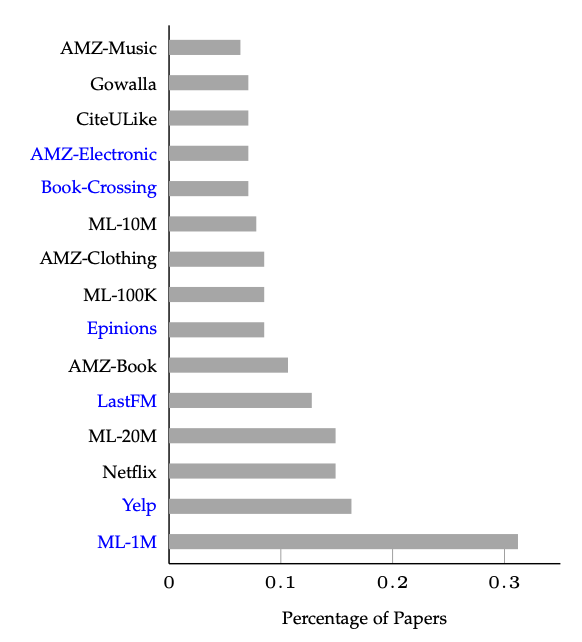
\includegraphics[width=0.6\textwidth]{images/dataset_dist.png}
    \caption{Розподіл використання наборів даних у наукових статтях.}
\end{figure}
Для практичних еспериментів, а також навчання і валідації моделей будо обрано відкриті набори даних які є загально прийняті і використовуються для порівняння у академічній сфері (Рис. 6.1). Для кожного датасету проведений розвідувальний аналіз даних (EDA) для оприділення їх основних структурних особливостей і відмінностей. Кожен набір є зрізом БД приватних комерційних компаній, тому можна вважати що поведінка моделей відповідає реальним результатам.

\subsubsection{Movielens 1M}
Набір даних Movielens (ML-1M) є найпопулярнішим серед великого різноманіття датасетів. Movielens -  це мережева система рекомендацій фільмів для користувачів на базі їх відгуків і оцінок. Існує із 1996 року і містить у собі більше 11 мільйонів оцінок для 8600 об’єктів.
\begin{figure}[H]
    \centering
    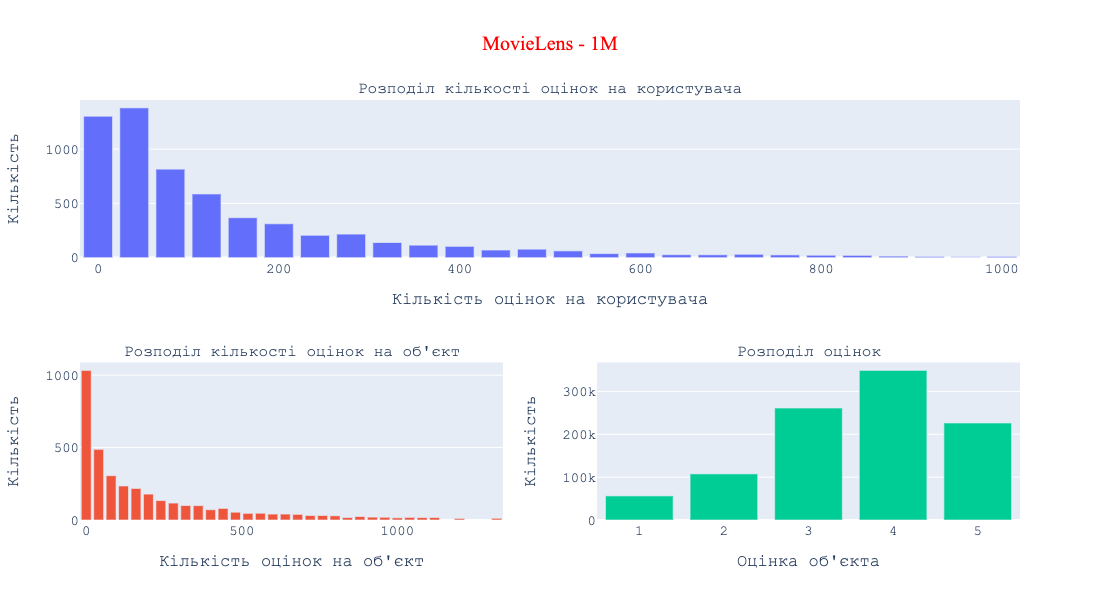
\includegraphics[width = 1\textwidth]{images/ML-1m_stat.png}    
    \caption{EDA для набору даних Movielens (ML-1M) }
\end{figure}
Структура набору наступна: 
\begin{itemize}
    \item $item\_id$ індентифікатор користувача.
    \item $user\_id$ індентифікатор об’єкта рекомендацій.
    \item $score$ оцінка.
    \item $timestamp$ дата і час дії.
\end{itemize}

Для аналізу відібрано 3706 об’єктів рекомендацій (фільмів) із 1 000 036  оцінок від корисутувачів. Що надає не менше 20 відгуків на один об’єкт.
\begin{table}[H]
    \centering
    \caption{Характеристика набору даних Movielens 1M}
    \begin{tabular}{|c|c|}
        \hline
        Загальна статистика      & Значення \\ \hline
        Кількість взаємодій      & 1 000 029                    \\
        Кількість користувачів   & 6 040                        \\
        Кількість об’єктів       & 3 706                        \\
        Розрідженність           & 99.9553\%                    \\
        Середня оцінка           & 3.58 / 5                     \\ \hline
        Взаємодій на користувача &                              \\ \hline
        Середнє                  & 165.6                        \\
        Медіана                  & 96.0                         \\ \hline
        Взаємодій на об’єкт      &                              \\ \hline
        Середнє                  & 269.89                       \\
        Медіана                  & 123.5                        \\ \hline
    \end{tabular}
    \label{tab:ML-1m}
\end{table}
Більшість оцінок приймають значення від 3 до 4-5. У розподілі взаємодій чітко замітний лівий перекіс, що типово для даних такого роду. Розрідженість висока.


\subsubsection{LastFm}
Набір даних LastFm містить у собі інформацію про музику яка прослуховується у медіа плеєрах користувачів. Структурно датасет подібний до ML-1M, але додатково присутня інформація про ключові теги класу для об’єктів. Теги можуть описувати жанр, автора, додаткову ключову інформацію, що є зручним і може бути використано для насичення моделей.


\begin{figure}[H]
    \centering
    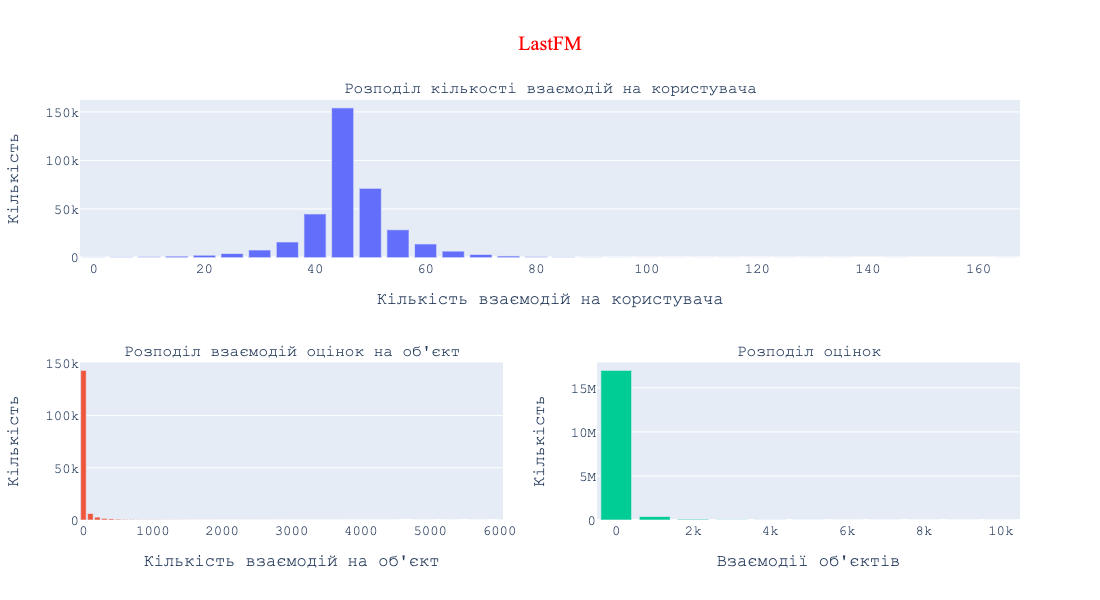
\includegraphics[width = 1\textwidth]{images/LastFM_stat.png}    
    \caption{EDA для набору даних Last.fm}
\end{figure}

\begin{table}[H]
    \centering
    \caption{Характеристика набору даних LastFM}
    \begin{tabular}{|c|c|}
        \hline
        Загальна статистика      & Значення \\ \hline
        Кількість взаємодій      & 17 535 654                    \\
        Кількість користувачів   & 358 868                        \\
        Кількість об’єктів       & 160 113                        \\
        Розрідженність           & 99.9996\%                    \\\hline
        Взаємодій на користувача &                              \\ \hline
        Середнє                  & 48.23                        \\
        Медіана                  & 48.0                         \\ \hline
        Взаємодій на об’єкт      &                              \\ \hline
        Середнє                  & 108.10                       \\
        Медіана                  & 6.0                        \\ \hline
    \end{tabular}

    \label{tab:LastFM}
\end{table}

\subsubsection{Netflix}
Набір даних Netflix є одним із найбільших відкритих датасетів із реальними даними. Набір був створений під егідою проведення змагання Netflix Prize. Ціллю якого було розробка системи рекомендацій, переможець який добився найвищих показників якості отримав призову винагороду у розмірі 1 мільйон доларів. Датасет має класичну структуру: включає у собі дані про оцінки користувачів фільмів які були переглянути користувачами. Для кожного екземпляру є відмітка про час оцінки. 

Дані мають типовий розподіл, і явно замітний перекіс. Із цікавого, через великий розмір і характер домену (рекомендація фільмів), датасет є одним із найнасичених. Розподіл оцінок - стандартний ([3, 4, 5]). Більше 90\% користувачів оцінили менше ста об’єктів.
\begin{figure}[H]
    \centering
    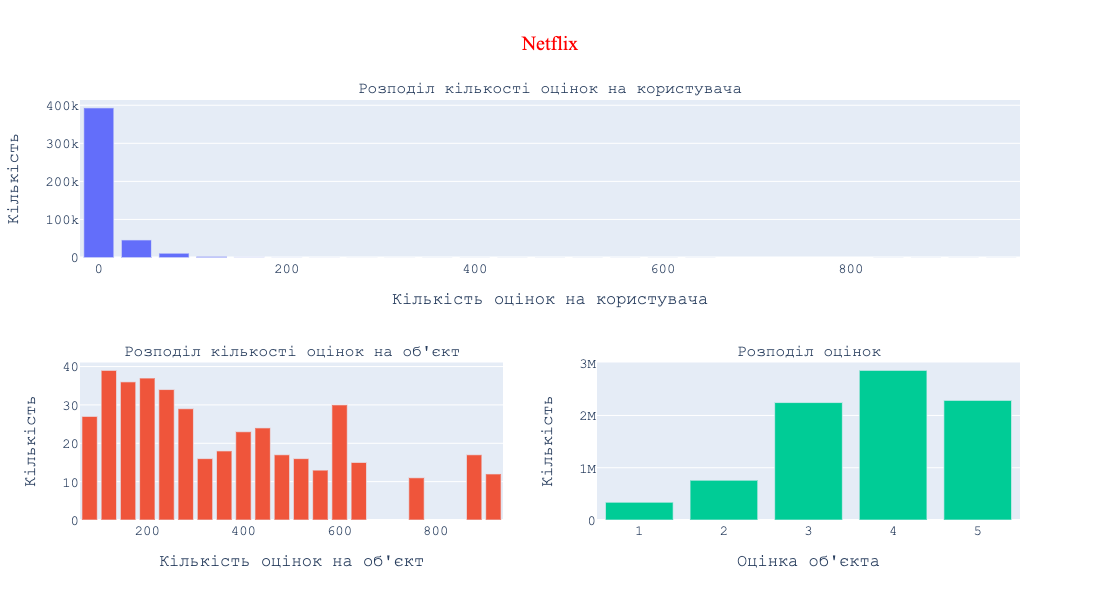
\includegraphics[width = 1\textwidth]{images/netflix_stat.png}    
    \caption{EDA для набору даних Netflix}
\end{figure}
У Таблиці 6.3 наведено докладна характеристика набору.
\begin{table}[H]
    \centering
    \caption{Характеристика набору даних Netflix}
    \begin{tabular}{|c|c|}
        \hline
        Загальна статистика      & Значення \\ \hline
        Кількість взаємодій      & 100 480 507                  \\
        Кількість користувачів   & 480 189                        \\
        Кількість об’єктів       & 17 770                        \\
        Розрідженність           & 98.8239\%                    \\\hline
        Взаємодій на користувача &                              \\ \hline
        Середнє                  & 209.33                       \\
        Медіана                  & 87.0                         \\ \hline
        Взаємодій на об’єкт      &                              \\ \hline
        Середнє                  & 5654.50                       \\
        Медіана                  & 967                      \\ \hline
    \end{tabular}
    \label{tab:Netflix}
\end{table}

Середня кількісь оцінок на об’єкт є надзвичайно високою.
\subsection{Середовище розгортання}

Експермиментальне дослідження проводиться на базі сервісу хмарних обчислень  Google Colab. Для навчання використано GPU Nvidia Tesla K80. Дані датасетів отримані із офіційних сторінок, розміщені у хмарному сховищі у вигляді текстових документів. Версія Python 3.8.15. Моделі імплементовані із використпанням бібліотеки torch. 

% Проведений аналіз наборів даних для побудови рекомендацій. Оцінено їх насиченість, частоту взаємодій відносно користувача і об’єкту. Наведено справочну інформацію про розмір, об’єм і структуру наборів. Вказано платформу реалізації практичних експериментів.

\subsection{Результати дослідження}
На основі аналізу факторів впливу, а також розглянутих перспективних нейромережевих моделей побудови рекомендацій було сформовано набір експериментів (Таблиця 8.1). Завдання експериментів, використовуючи набори даних, які відповідають реальним вибіркам із БД комерційних компаній дослідити вплив широкого спектру розглянутих факторів. Використовуючи мову програмування Python, а також платформу хмарних обчислень Google Coolab імплементувано розглянуті алгоритми Neural Matrix Factorization, Variational AutoEncoder ,  Neural Graph Colaborative Filtering.

На основі імплементованих алгоритмів проведений порівняльний аналіз ефективності використовуючи метрики вказані у Таблиці 8.1 . 
% Провести пошук оптимальних гіперпараметрів для алгоритмів. Розглянути еффективіність методів:
% \begin{itemize}
%     \item Сплітингу
%     \item Семплювання
%     \item Ініціалізації гіперпараметрів
%     \item Оптимізації
%     \item Регуляризації
% \end{itemize}

% \begin{table}[h]
%     \caption{}
%     \begin{tabular}{|c|c|}
%         \hline
%         Фактор                 & Значення                                                                                   \\ \hline
%         Датасет                & ML-1m, LastFM, Netflix                                                                     \\ \hline
%         Модель                 & NeuMF, VAE, NGCF                                                                           \\ \hline
%         Фільтрація датасету    & Без фільтрації, 5, 10                                                                      \\ \hline
%         Сплітінг датасету      & За пропорціями, За часом                                                                   \\ \hline
%         Метрик оцінки якості   & \begin{tabular}[c]{@{}c@{}}Precision@k, Recall@k, MAP, HitRatio, MRR, \\ NDCG\end{tabular} \\ \hline
%         Семплювання            & Розподіл Гауса, low popularity, high popularity                                            \\ \hline
%         Ініціалізація $\theta$ & Рівномірний розподіл, Розподіл Гауса                                                       \\ \hline
%         Метод оптимізації      & GD, SGD, BSGD, AdaGrad, RMSProp                                                            \\ \hline
%         Регуляризація          &                                                                                            \\ \hline
%         Підбір гіперпараметрів & GridSearch, Bayesian HyperOpt                                                              \\ \hline
%     \end{tabular}
%     \label{tab:Expr_design}
% \end{table}

\begin{table}[h]
    \caption{Деталі експерименту}
    \begin{tabular}{|c|c|}
        \hline
        Фактор                 & Значення                                                                                   \\ \hline
        Датасет                & ML-1m, LastFM, Netflix                                                                     \\ \hline
        Модель                 & NeuMF, VAE, NGCF                                                                           \\ \hline
        Фільтрація датасету    & Без фільтрації                              \\ \hline
        Сплітінг датасету      & За часом                                                                   \\ \hline
        Метрик оцінки якості   & \begin{tabular}[c]{@{}c@{}}Precision@k, Recall@k, MAP, HitRatio, MRR, \\ NDCG\end{tabular} \\ \hline
        Семплювання            & Розподіл Гауса                                            \\ \hline
        Ініціалізація $\theta$ &  Розподіл Гауса                                                       \\ \hline
        Метод оптимізації      &  AdaGrad                                                             \\ \hline
        Регуляризація          &  L2                                                                                          \\ \hline
        Підбір гіперпараметрів & GridSearch                                                              \\ \hline
    \end{tabular}
    \label{tab:Expr_design}
\end{table}
Значення функцій втрат під час навчання для кожного із алгоритмів вказано на Рис. 8.1. Для NeuMF  було застосовано ранню зупинку, loss не змінювався протягом 3 епох. Дельта втрат вказує на рівномірне зменшування функції втрат.
Для MultiVAE доцільно використати сильнішу регуляризацію. 
\begin{figure}
    \begin{subfigure}{\textwidth}
        \centering
        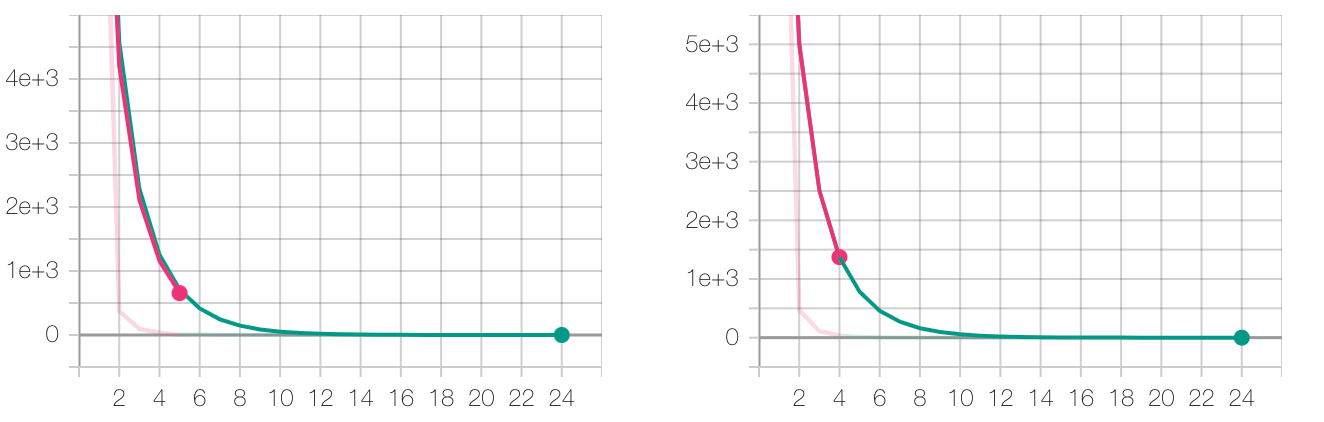
\includegraphics[width=.5\textwidth]{images/experiments/neumf_loss.png}
        \caption{Навчання NeuMF на 24 епохах}
    \end{subfigure}
    \begin{subfigure}{\textwidth}
        \centering
        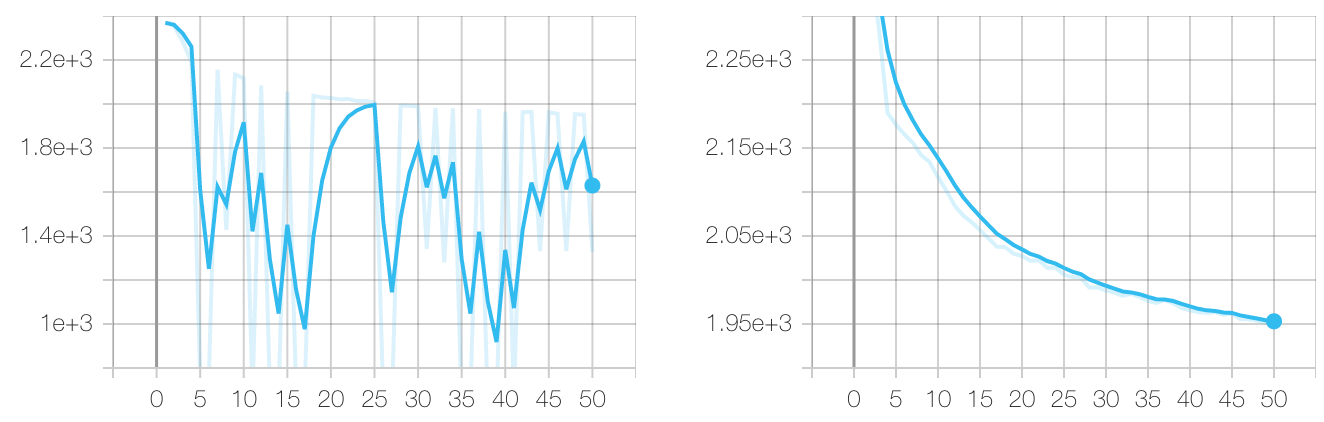
\includegraphics[width=.5\textwidth]{images/experiments/multivae_loss.png}
        \caption{Навчання MultiVae на 50 епохах}
    \end{subfigure}
    \begin{subfigure}{\textwidth}
        \centering
        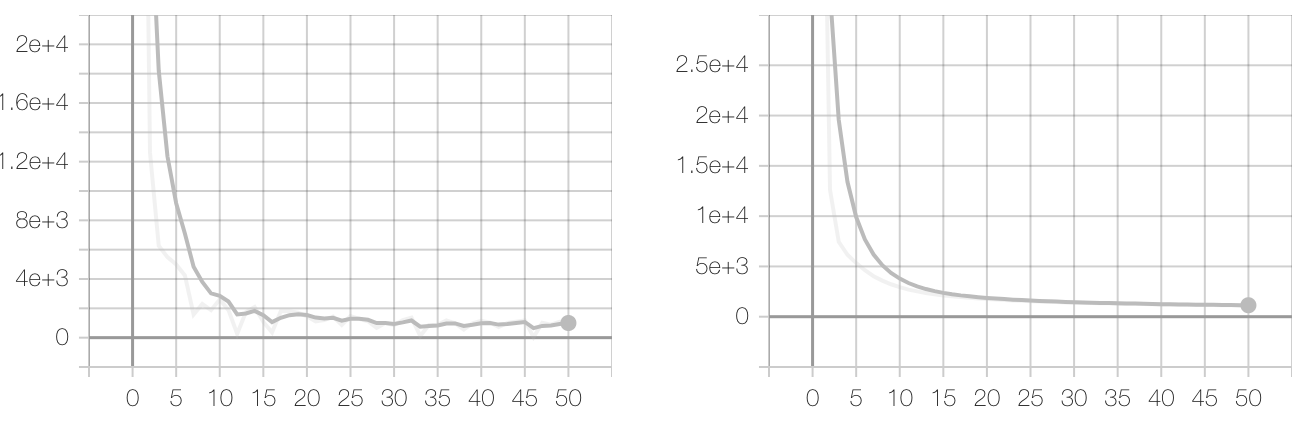
\includegraphics[width=.5\textwidth]{images/experiments/ngcd_loss.png}
        \caption{Навчання NGCF на 50 епохах}
    \end{subfigure}
    \caption{Процес навчання алгоритмів. Зправа - Значення функції втрат, Зліва - дельта втрат відносно епохи.}
\end{figure}
У наступних таблицях вказано результи метри якості розраховані на наборі даних Movielens.  K (розмір списку рекомендацій) був обраний із інтервалу [1, 50].
Для розрахунку бува використане негативне семплювання, із розміро вибірки 1000 у кандидатів.
\begin{table}
    \centering
    \begin{tabular}{|l|l|l|l|l|l|l|}
        \hline
        KPI@K     & 1       & 5       & 10     & 20     & 30     & 50     \\ \hline
        Recall    & 0.01452 & 0.06699 & 0.1235 & 0.2215 & 0.3012 & 0.4135 \\ \hline
        MRR       & 0.6961  & 0.7929  & 0.79   & 0.7981 & 0.7983 & 0.7985 \\ \hline
        NDCG      & 0.6961  & 0.8175  & 0.8200 & 0.8112 & 0.8050 & 0.7978 \\ \hline
        Hit Ratio & 0.6961  & 0.9246  & 0.9584 & 0.9636 & 0.9688 & 0.9766 \\ \hline
        Precision & 0.6961  & 0.641   & 0.5906 & 0.5302 & 0.4785 & 0.3966 \\ \hline
    \end{tabular}
    \caption{Значення метрик якості для алгоритму MultiVAE. Набір даних MovieLens}
\end{table}
\begin{table}
    \begin{tabular}{|l|l|l|l|l|l|l|}
        \hline
        KPI@K     & 1        & 5        & 10      & 20      & 30      & 50      \\ \hline
        Recall    & 0.001757 & 0.008701 & 0.01956 & 0.02799 & 0.04172 & 0.05583 \\ \hline
        MRR       & 0.04318  & 0.07580  & 0.0839  & 0.0901  & 0.09206 & 0.0941  \\ \hline
        NDCG      & 0.04318  & 0.08929  & 0.1087  & 0.1315  & 0.1407  & 0.157   \\ \hline
        Hit Ratio & 0.04318  & 0.1295   & 0.1926  & 0.2823  & 0.3322  & 0.4086  \\ \hline
        Precision & 0.04318  & 0.04518  & 0.04186 & 0.03787 & 0.03665 & 0.03342 \\ \hline
    \end{tabular}
    \caption{Значення метрик якості для алгоритму NGCF. Набір даних MovieLens}
\end{table}
\begin{table}
    \begin{tabular}{|l|l|l|l|l|l|l|}
        \hline
        KPI@K     & 1        & 5       & 10      & 20      & 30     & 50      \\ \hline
        Recall    & 0.003363 & 0.01157 & 0.02017 & 0.04535 & 0.0611 & 0.09025 \\ \hline
        MRR       & 0.1694   & 0.2382  & 0.2603  & 0.2688  & 0.2717 & 0.2732  \\ \hline
        NDCG      & 0.1694   & 0.2688  & 0.322   & 0.354   & 0.3701 & 0.381   \\ \hline
        Hit Ratio & 0.1694   & 0.365   & 0.5348  & 0.657   & 0.73   & 0.7873  \\ \hline
        Precision & 0.1694   & 0.1408  & 0.1355  & 0.1250  & 0.119  & 0.1136  \\ \hline
    \end{tabular}
    \caption{Значення метрик якості для алгоритму NeuMF. Набір даних MovieLens}
\end{table}

\begin{figure}[H]
    \centering
    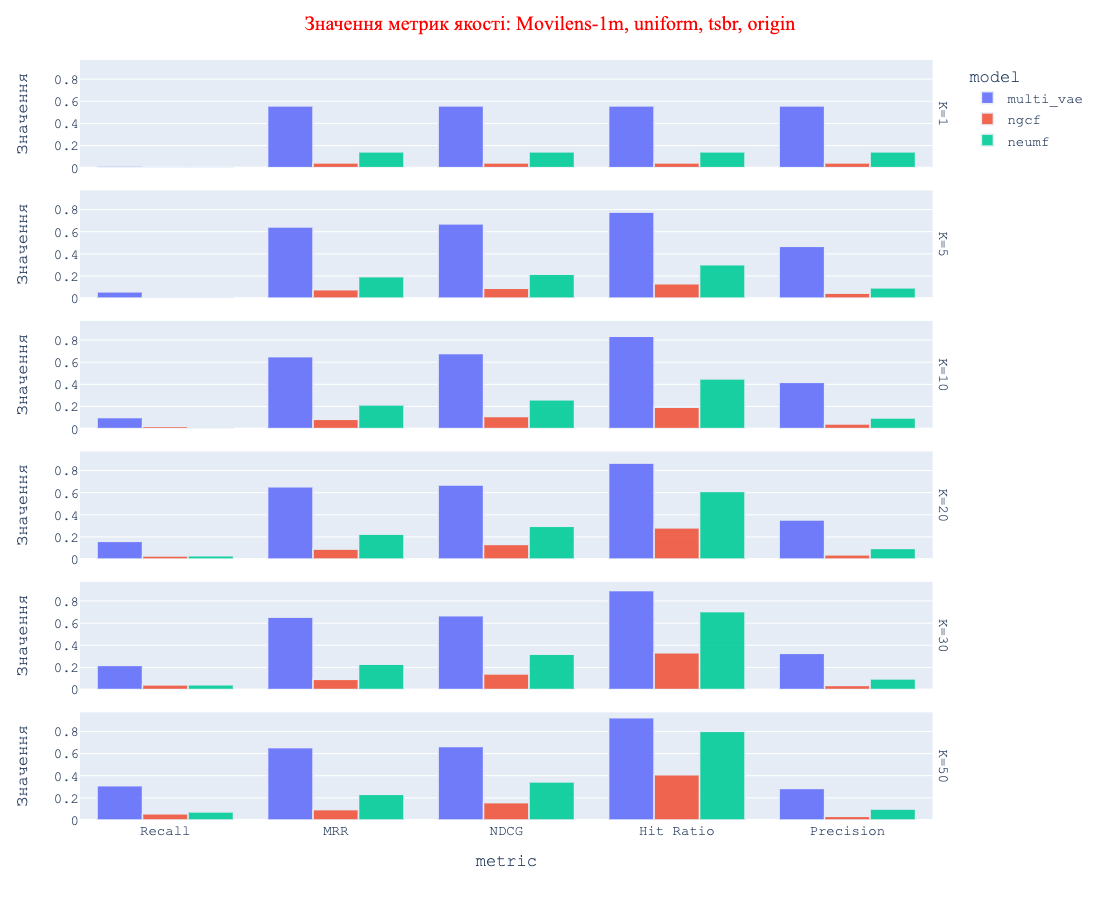
\includegraphics[width=1\textwidth]{images/experiments/metrics_exp_1.png}
    \caption{Порівняльний графік метрик якості}
\end{figure}

Алгоритм MultiVae  показав найвищі показники метрик якості на усіх вибірках K,. Варіаційний автоенкодер показує потужну властивість до вивчення поведінки користувачів.


\subsection*{Висновки}
Було проведено експерементальне дослідження здатності до побудови рекомендацій алгоритмів NueMF, MultiVAE і NGCF. За результатами тестування,  MultiVAE  показав найвищі результати по всім розглянутим метрикам.